\usepackage{etoolbox}
\usepackage{ifthen}

% Put this file into the preamble and call it via
% \input{tikzdice.tex}
%
% Jesse Hamner
% https://github.com/jessehamner/tikzdice
% 2020


\usetikzlibrary{arrows}

\tikzset{
  treenode/.style = {align=center, text centered,
    font=\sffamily},
  arn_n/.style = {treenode, font=\sffamily\bfseries, draw=black,
    fill=black, text width=1.5em},
  arn_r/.style = {treenode, text width=1.5em},
  arn_x/.style = {treenode, minimum width=0.5em, minimum height=0.5em}
}

\newcommand{\majelaxis}{0.5}
\newcommand{\minelaxis}{0.125}

\newcommand{\headtext}{\color{red}\textbf{H}}

\newcommand{\dieone}{\maindie{1}{0}}
\newcommand{\dietwo}{\maindie{2}{0}}
\newcommand{\diethree}{\maindie{3}{0}}
\newcommand{\diefour}{\maindie{4}{0}}
\newcommand{\diefive}{\maindie{5}{0}}
\newcommand{\diesix}{\maindie{6}{0}}

\newcommand{\pipsize}{3.05pt}
\newcommand{\diecolor}{red}
\newcommand{\pipcolor}{red}
\newcommand{\fieldfill}{white}

\newcommand{\piplocation}[2]{\filldraw[fill=\pipcolor] (#1,#2) circle (\pipsize);}

\newcommand{\piplocationone}{\piplocation{0.25}{0.25}}
\newcommand{\piplocationtwo}{\piplocation{0.50}{0.25}}
\newcommand{\piplocationthree}{\piplocation{0.75}{0.25}}
\newcommand{\piplocationfour}{\piplocation{0.25}{0.50}}
\newcommand{\piplocationfive}{\piplocation{0.50}{0.50}}
\newcommand{\piplocationsix}{\piplocation{0.75}{0.50}}
\newcommand{\piplocationseven}{\piplocation{0.25}{0.75}}
\newcommand{\piplocationeight}{\piplocation{0.50}{0.75}}
\newcommand{\piplocationnine}{\piplocation{0.75}{0.75}}

\newcommand{\spreadsix}{\piplocation{0.20}{0.20}\piplocation{0.20}{0.80}
						\piplocation{0.80}{0.20}\piplocation{0.80}{0.80}
						\piplocation{0.50}{0.20}\piplocation{0.50}{0.80}}

\newcommand{\maindie}[2]{
\ifthenelse{#2 = 0}{\renewcommand{\diecolor}{black}\renewcommand{\pipcolor}{black}\renewcommand{\fieldfill}{white}}{}%
\ifthenelse{#2 = 1}{\renewcommand{\diecolor}{red}\renewcommand{\pipcolor}{red}\renewcommand{\fieldfill}{white}}{}%
\ifthenelse{#2 = 2}{\renewcommand{\diecolor}{blue}\renewcommand{\pipcolor}{blue}\renewcommand{\fieldfill}{white}}{}%
\ifthenelse{#2 = 3}{\renewcommand{\diecolor}{black}\renewcommand{\pipcolor}{white}\renewcommand{\fieldfill}{black}}{}%
\begin{tikzpicture}
  \draw[very thick, rounded corners, \diecolor, fill=\fieldfill] (0,0) rectangle (1,1);
  \ifthenelse{#1 = 1}{\piplocationfive}{}%
  \ifthenelse{#1 = 2}{\piplocationone\piplocationnine}{}%
  \ifthenelse{#1 = 3}{\piplocationone\piplocationfive\piplocationnine}{}%
  \ifthenelse{#1 = 4}{\piplocationone\piplocationnine\piplocationthree\piplocationseven}{}%
  \ifthenelse{#1 = 5}{\piplocationone\piplocationnine\piplocationthree\piplocationseven\piplocationfive}{}%
  \ifthenelse{#1 = 6}{\piplocation{0.20}{0.25}\piplocation{0.20}{0.75}
					  \piplocation{0.80}{0.25}\piplocation{0.80}{0.75}
					  \piplocation{0.20}{0.50}\piplocation{0.80}{0.50}}{}%

  \ifthenelse{#1 = 7}{\spreadsix\piplocationfive}{}%
  \ifthenelse{#1 = 8}{\spreadsix\piplocation{0.20}{0.50}\piplocation{0.80}{0.50}}{}%
  \ifthenelse{#1 = 9}{\spreadsix\piplocation{0.20}{0.50}\piplocation{0.80}{0.50}\piplocationfive}{}%
  \ifthenelse{#1 = 0}{}{}%
%    \ifthenelse{#1 = 0}{\draw[very thick, rounded corners, \diecolor, fill=\diecolor!20] (0,0) rectangle (1,1);}{}%

\end{tikzpicture}
}


\pgfmathdeclarefunction{addone}{1}{
  \pgfmathparse{#1 + \majelaxis}
}

\pgfmathdeclarefunction{addtwo}{1}{
  \pgfmathparse{#1 + \majelaxis + \majelaxis}
}

\pgfmathdeclarefunction{addspace}{1}{
  \pgfmathparse{#1 + 1.15}
}


\newcommand{\coin}[4]{
  \pgfmathsetmacro{\argthree}{addone(#1)}
  \pgfmathsetmacro{\argtwo}{addtwo(#1)}

  \shade[left color=white, right color=black]
    ({\argthree},0mm) ellipse (\majelaxis cm and \minelaxis cm);
  \shade[left color=white, right color=black]
    ({#1},0mm) rectangle (\argtwo cm, 1mm);

  \draw({\argthree},0.5cm) node[color=blue, above]{#2};

  \draw[fill=#4]({\argthree},1mm) ellipse (\majelaxis cm and \minelaxis cm);
  \draw ({#1},0mm) arc (180:360:\majelaxis cm and \minelaxis cm);
  \draw({#1},0mm) -- ({#1}, 1mm);
  \draw({\argtwo},0mm) -- ({\argtwo}, 1mm);

  \draw({\argthree},-0.4cm) node[color=black, below]{#3};
}

\newcommand{\heads}[2]{
\coin{#1}{#2}{\headtext}{blue!50}
}

\newcommand{\tails}[2]{
\coin{#1}{#2}{{\color{gray!70}T}}{white}
}




\newcommand{\wtf}{\theheadpos & \makecoinrow{} \\}

\newcommand{\whichheads}{1}
\newcounter{num}
\setcounter{num}{1}
\newcounter{headpos}
\setcounter{headpos}{1}
\newcounter{int}
\setcounter{int}{1}


% Row of coins, one head, slot #1.

\newcommand{\makecoinrow}{
  \setcounter{int}{1}

  \begin{tikzpicture}[]
    \newdimen\R
    \R=0cm

    \loop
      \ifthenelse{\value{int}=\value{headpos}}{\heads{\R}{}}{\tails{\R}{}}
      \pgfmathsetmacro{\R}{addspace(\R)}
      \stepcounter{int}
      \ifnum \value{int}<11
    \repeat

  \end{tikzpicture}

  \smallskip
}



% Definition of circles and square
\def\firstcircle{(0,0) circle (1.5cm)}
\def\secondcircle{(2,0) circle (1.5cm)}
\def\firstsquare{(-1.6,-1.6) rectangle (1.6,1.6)}


\def\missed{\LARGE\textbf{X}}
\def\target{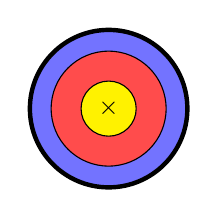
\begin{tikzpicture}
  \draw[ultra thick, black, fill=blue!55] (0,0) circle(1cm);
  \draw[fill=red!70] (0,0) circle(0.73cm);
  \draw[fill=yellow] (0,0) circle(0.35cm) node{\small$\times$};
\end{tikzpicture}}

% Set colors
\colorlet{circle edge}{blue!50}
\colorlet{circle area}{blue!20}
\colorlet{rectangle edge}{blue!50}
\colorlet{rectangle area}{blue!20}

\tikzset{filled/.style={fill=circle area, draw=circle edge, thick},
    	 outline/.style={draw=circle edge, thick}
	    }
% This line makes makes theorems and boxed environments align incorrectly (vertically) in Beamer, I suggest that you remove it
% \setlength{\parskip}{5mm}

% This command is a nice shortcut in my opinion that makes the dice aligned vertically when they're used with text or in math mode.
% Possibly you want to use another (optional?) argument for the scalebox parameter to tune the size
\newcommand\vcdice[2]{\vcenter{\hbox{\scalebox{0.4}{\maindie{#1}{#2}}}}}



\def\missed{\LARGE\textbf{X}}
\def\target{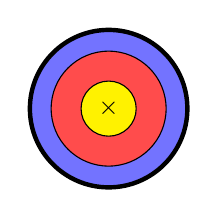
\begin{tikzpicture}
  \draw[ultra thick, black, fill=blue!55] (0,0) circle(1cm);
  \draw[fill=red!70] (0,0) circle(0.73cm);
  \draw[fill=yellow] (0,0) circle(0.35cm) node{\small$\times$};
\end{tikzpicture}}

\tikzset{
  treenode/.style = {align=center, text centered, font=\sffamily},
  arn_n/.style = {treenode, font=\sffamily\bfseries, draw=black, fill=black},
  arn_r/.style = {treenode},
  arn_x/.style = {treenode}
}
